\documentclass[11pt,a4paper]{article}

\usepackage[margin=1in]{geometry}
\usepackage{amsmath,amssymb,amsthm}
\usepackage{mathtools}
\usepackage{hyperref}
\usepackage{booktabs}
\usepackage{longtable}
\usepackage{array}
\usepackage{tikz}
\usetikzlibrary{arrows.meta,positioning}
\usepackage{enumitem}

\hypersetup{
  colorlinks=true,
  linkcolor=blue!50!black,
  citecolor=blue!50!black,
  urlcolor=blue!60!black
}

\newtheorem{conjecture}{Conjecture}
\newtheorem{problem}{Open Problem}
\theoremstyle{definition}
\newtheorem{definition}[conjecture]{Definition}
\theoremstyle{remark}
\newtheorem{remark}[conjecture]{Remark}

\newcommand{\PSLZ}{\mathrm{PSL}_2(\mathbb{Z})}
\newcommand{\PCF}{\mathrm{PCF}}
\newcommand{\Q}{\mathbb{Q}}
\newcommand{\Z}{\mathbb{Z}}
\newcommand{\R}{\mathbb{R}}
\newcommand{\C}{\mathbb{C}}
\newcommand{\OO}{\mathcal{O}}
\newcommand{\HH}{\mathfrak{H}}
\newcommand{\PetN}[1]{\lVert #1 \rVert_{\mathrm{Pet}}}

\title{An Arithmetic Stratification of Polynomial Continued Fractions:\\
       Program Statement of the SIARC Series\\
       \large (v2.0: Modular-Discriminant Framing)}
\author{papanokechi}
\date{May 2026}

\begin{document}
\maketitle

\begin{abstract}
This paper is a \emph{program statement}, not a results paper. It is the
v2.0 revision of the SIARC umbrella program statement, refactoring the
v1 (April 2026) framing around a cross-degree \emph{invariant triple}
\(\bigl(\Delta_d(b),\ \PetN{\Delta}(\tau_b),\ \xi_0(b)\bigr)\) that
emerged from the SIARC stack between v1 and v2. The triple combines
the polynomial discriminant of the denominator polynomial \(b\) (the
discriminant axis), the Petersson-normalised modular discriminant
evaluated at the period \(\tau_b\) of the curve \(y^2 = b(x)\) (the
modular-discriminant axis), and the Newton-polygon Borel radius
\(\xi_0(b) = d/\beta_d^{1/d}\) (the Borel-radius axis). v2.0 integrates
the four sister Zenodo records published since v1 --- PCF-1 v1.3,
PCF-2 v1.3, Channel Theory v1.2, and the standalone j-invariant
note --- into a single cross-degree organisational scheme, retains the
$\PSLZ$ four-tier hierarchy at degree pair \((2,1)\) as the d=2
specialisation, and refreshes the Open Problems list with the
post-T2 entries (\textsf{op:j-zero-amplitude-h6},
\textsf{op:j-1728-wedge}, \textsf{op:shallow-j-effect-d4},
\textsf{op:b4-degree-d}, \textsf{op:median-resurgence-extension}).
\emph{No proofs and no new theorems are reproduced here}; every
nontrivial claim is stated as a conjecture or attached to a companion
paper by Zenodo DOI. The purpose of this document is to provide a
stable, citable scope-anchor (\emph{[SIARC v2.0]}) for the program
and to fix unified notation for the post-March 2026 stack.
\end{abstract}

\tableofcontents

\section{Introduction and Motivation}
\label{sec:intro}

A \emph{polynomial continued fraction} (PCF) is a formal continued fraction
\begin{equation}
  \label{eq:pcf-def}
  K(x) \;=\; b_0(x) + \cfrac{a_1(x)}{b_1(x) + \cfrac{a_2(x)}{b_2(x) + \cfrac{a_3(x)}{b_3(x) + \ddots}}}
\end{equation}
in which the partial numerators $a_n(x)$ and partial denominators $b_n(x)$
are fixed polynomials in $x$ with integer (or rational) coefficients, evaluated
at a fixed integer $x \in \Z_{\geq 1}$. The classical Ramanujan and
Rogers--Ramanujan continued fractions, the Stern--Brocot expansions of
quadratic irrationals, and the Apéry-style recurrences for $\zeta(2)$ and
$\zeta(3)$ are all PCFs in this sense. A central problem, going back to
Stieltjes and revisited in the modern era by Lagarias, Borwein, and others,
is to determine the \emph{arithmetic nature} of the limit of \eqref{eq:pcf-def}:
when is it rational, when is it algebraic, when is it transcendental, and
when does it fail to converge to a number that admits any such classification?

The SIARC program proposes that this arithmetic question is not
homogeneous. PCFs admit a natural \emph{stratification} indexed by
(i) the uniformizing Fuchsian group of the associated monodromy
representation, and (ii) an obstruction tier that records how far the
limit lies from being algebraic over $\Q$. This stratification organizes
otherwise unrelated empirical phenomena --- the appearance of $-2/9$
exponents in degree-$(2,1)$ families, the Painlevé connection in
degree-$(3,1)$ families, the failure of the Mahler criterion at
specific lattice points --- into a single arithmetic picture.

\paragraph{Goal of the program.}
The SIARC program aims to define, for each Fuchsian group $\Gamma$ that
arises as a uniformizer of a PCF family, a four-tier arithmetic
stratification (\S\ref{sec:tiers}), to verify the stratification on the
$\PSLZ$ case completely (companion paper \#14), and to extend it
conjecturally to the remaining classical groups via the Trans-Stratum
Conjecture (\S\ref{sec:t2b}) and the open problems of \S\ref{sec:open}.

\paragraph{What changed between v1 and v2.0.}
\label{par:v1-to-v2}
v1 (Zenodo concept DOI \href{https://doi.org/10.5281/zenodo.19885550}{10.5281/zenodo.19885550})
organised PCFs by (Fuchsian group, tier), anchored in $\PSLZ$ and the
degree pair $(2,1)$. Between v1 and v2.0 the SIARC stack produced four
companion records that demand a cross-degree organisational principle:
PCF-1 v1.3 (sharp WKB exponents at $d=2$ stratified by $\mathrm{sgn}(\Delta_2)$),
PCF-2 v1.3 (a cubic-modular framing at $d=3$),
Channel Theory v1.2 (a Borel-resurgence functor on the V$_{\mathrm{quad}}$
stratum), and a standalone j-invariant note (the equianharmonic cubic
cell). v2.0 reorganises the umbrella around the \emph{invariant triple}
\begin{equation}
  \label{eq:invariant-triple}
  \PCF(1,b) \;\longmapsto\; \bigl(\Delta_d(b),\ \PetN{\Delta}(\tau_b),\ \xi_0(b)\bigr),
\end{equation}
introduced in \S\ref{sec:triple}. The two pictures are
\emph{compatible}: at $d=2$ the triple-invariant framing recovers the
$\PSLZ$ four-tier hierarchy of v1 as the $\Delta_2$-axis split with
trivial $\PetN{\Delta}$-axis, and the Trans-Stratum two-class
conjecture of \S\ref{sec:t2b} reappears as the Class A / Class B
dichotomy at $d=2$. At $d \geq 3$ the triple is genuinely new
information; the four-tier hierarchy extends \emph{conjecturally},
with empirical support from PCF-2 v1.3.

\section{The Four-Tier Hierarchy}
\label{sec:tiers}

We summarize the tier definitions. Full proofs of the classification
theorem are deferred to the $\PSLZ$ paper; see Remark~\ref{rem:tiers-source}.

\begin{definition}[Tier T0: Algebraic]
A PCF family $\{K(x)\}_{x \in S}$ lies in tier T0 over an arithmetic set
$S \subseteq \Z_{\geq 1}$ if $K(x)$ is algebraic over $\Q$ for every
$x \in S$, and the algebraic degree is uniformly bounded as $x$ varies in $S$.
\end{definition}

\begin{definition}[Tier T1: Transcendental]
A PCF family lies in tier T1 if $K(x)$ is transcendental for every $x \in S$,
\emph{and} a Mahler-type or Nesterenko-type criterion certifies the
transcendence uniformly in $x$.
\end{definition}

\begin{definition}[Tier T2: Trans-stratum]
A PCF family lies in tier T2 if its irrationality measure $\mu(K(x))$
satisfies an asymptotic
\[
   \mu(K(x)) \;=\; 2 + \frac{c}{\log x} + o\!\left(\frac{1}{\log x}\right),
   \qquad x \to \infty,
\]
for an explicit rational constant $c$ (the \emph{trans-stratum exponent})
that depends only on the polynomial degrees $(\deg a, \deg b)$ and the
Fuchsian group $\Gamma$. The trans-stratum is therefore not a transcendence
statement, but a statement about the rate at which transcendence is
approached.
\end{definition}

\begin{definition}[Tier T3: Barrier]
A PCF family lies in tier T3 if the Fuchsian uniformization itself
degenerates: either $\Gamma$ fails to be of finite covolume, or the
associated $L$-function fails to admit analytic continuation to the
required half-plane. T3 families are inaccessible to the methods of T0--T2
and serve as the negative boundary of the program.
\end{definition}

\begin{remark}[Translation to the obstruction hierarchy of \#14]
\label{rem:tier-translation}
The companion paper~\#14 introduces a parallel four-tier
\emph{obstruction} hierarchy $O_0,\dots,O_3$ measuring the
distance from the modular sector $X(1)$. The two
hierarchies do not coincide. We have the inclusions
$O_0 \subseteq T_0 \cup T_2$, $O_1 \subseteq T_2$,
$O_2 \subseteq T_2$, $O_3 \subseteq T_3$, but in general
neither family of tiers refines the other. We use $T_0,\dots,T_3$
exclusively for the arithmetic hierarchy of this paper, and
$O_0,\dots,O_3$ for the obstruction hierarchy of~\#14.
\end{remark}

\begin{remark}[Source of the classification]
\label{rem:tiers-source}
A full classification theorem stating that every $\PSLZ$-uniformized
PCF family lies in exactly one of T0, T1, T2, T3 --- and that the
tier is computable from $(\deg a, \deg b)$ and the leading coefficients
--- is the main theorem of companion paper \#14. We do not reproduce
either the statement in full generality or the proof here. See the
companion paper table in \S\ref{sec:companions}.
\end{remark}

\paragraph{Forward reference to the cross-degree framing.}
\label{par:forward-ref-triple}
The four tiers above are stated for $\PSLZ$-uniformized families at
degree pair $(2,1)$. Their behaviour at degree $d \geq 3$ is the subject
of the cross-degree framing of \S\ref{sec:triple}: the discriminant axis
$\Delta_d$ refines the T0/T1 boundary at every $d$ (PCF-1 v1.3
Theorem~5; \cite{PCF1}); the modular-discriminant axis $\PetN{\Delta}$
refines the T2 stratum at $d=3$ (PCF-2 v1.3 Conjectures B5/B6;
\cite{PCF2}); the Borel-radius axis $\xi_0$ refines the T3 boundary
via Newton-polygon resurgence (Channel Theory v1.2; \cite{CT}). The
v1 four-tier hierarchy is the d=2, $\Delta_2$-only specialisation of
the cross-degree picture.

\section{Cross-Degree Framing: the Invariant Triple}
\label{sec:triple}

This section is new in v2.0. It records the cross-degree
organisational principle that emerged from the SIARC stack between
April and May 2026. \emph{No new theorems are stated here}; every
quantitative claim is either empirical (with citation to the responsible
companion paper's session deliverables) or conjectural.

\subsection{Definitions}
\label{sec:triple-defs}

Throughout this section, fix a PCF family of the form
$\PCF(1, b) = 1/(b_1 + 1/(b_2 + \cdots))$ with $b_n = b(n)$ for a fixed
polynomial $b \in \Q[x]$ of degree $d$. Write
$b(x) = \beta_d x^d + \beta_{d-1} x^{d-1} + \cdots + \beta_0$.

\begin{definition}[Discriminant axis]
\label{def:disc-axis}
The \emph{discriminant} of $b$ is $\Delta_d(b) := \mathrm{disc}(b)$, the
ordinary polynomial discriminant of the squarefree-part-stripped
denominator polynomial. By convention $\Delta_d(b) \in \Q^\times$ when
$b$ is squarefree, and the sign $\mathrm{sgn}(\Delta_d) \in \{\pm 1\}$
is the discrete invariant on which PCF-1 v1.3 stratifies the sharp
WKB exponent at $d=2$.
\end{definition}

\begin{definition}[Modular-discriminant axis]
\label{def:moddisc-axis}
For $d=3$ with $b$ irreducible non-singular, the curve $E_b: y^2 = b(x)$
is an elliptic curve over $\Q$; let $\tau_b \in \HH/\mathrm{SL}_2(\Z)$
be its period in the standard fundamental domain. The
\emph{Petersson-normalised modular discriminant} at $\tau_b$ is
\begin{equation}
  \label{eq:petersson-norm}
  \PetN{\Delta}(\tau_b) \;:=\; |\Delta(\tau_b)| \cdot (\mathrm{Im}\,\tau_b)^{6},
\end{equation}
where $\Delta(\tau) = (2\pi)^{12} \eta(\tau)^{24}$ is the modular
discriminant cusp form of weight $12$. For general $d \geq 3$ the
analogous construction uses the period of the hyperelliptic curve
$y^2 = b(x)$ on the corresponding period domain; we restrict the
quantitative claims of this section to $d=3$.
\end{definition}

\begin{definition}[Borel-radius axis]
\label{def:borel-axis}
The \emph{Borel radius} of the PCF asymptotic series associated to
$\PCF(1,b)$ is
\begin{equation}
  \label{eq:borel-radius}
  \xi_0(b) \;:=\; \frac{d}{\beta_d^{1/d}},
\end{equation}
the Newton-polygon root extracted from the dominant balance of the
characteristic equation of the three-term recurrence at infinity
(\cite{PCF2}, Q1-B Proposition; \cite{CT}, V$_{\mathrm{quad}}$
recovery).
\end{definition}

The map
\begin{equation}
  \label{eq:Phi-functor}
  \Phi : \PCF(1,b) \;\longmapsto\; \bigl(\Delta_d(b),\ \PetN{\Delta}(\tau_b),\ \xi_0(b)\bigr)
\end{equation}
is the \emph{bridge functor} of v2.0; the rest of this section reviews
what each axis carries.

\subsection{The discriminant axis \texorpdfstring{$\Delta_d$}{Delta\_d}}
\label{sec:triple-disc}

At $d=2$, PCF-1 v1.3 Theorem~5 establishes the sharp WKB exponent
identity for $\PCF(1,b)$ with $\deg b = 2$, with the exponent split by
$\mathrm{sgn}(\Delta_2)$: $A = 4$ for $\Delta_2 > 0$ and $A = 3$ for
$\Delta_2 < 0$ (six $\Delta_2 < 0$ families verified at $\geq 200$
digits; see PCF-1 v1.3 \cite{PCF1}). At $d \geq 3$, PCF-2 v1.3
\cite{PCF2} verifies the unsplit \emph{sharp} Conjecture B4
\begin{equation}
  \label{eq:b4-conjecture}
  \log|\delta_n| \;\sim\; -A\, n \log n + \alpha\, n - \beta \log n + \gamma,
  \qquad A = 2d
\end{equation}
on the joint $d \in \{3,4\}$ catalogue (110/110 families at the
relevant tail-window precision). The strong-form upgrade
\textsf{op:b4-degree-d} (\S\ref{sec:open}, \textsf{prob:b4-allD})
extends $A = 2d$ to all $d$ via the Birkhoff--Trjitzinsky
asymptotic theory of irregular linear difference equations
\cite{Birkhoff1930,BirkhoffTrjitzinsky1933}; this remains open and is
the gating move toward the \emph{SIARC Master Conjecture v0}
(MASTER-V0, \S\ref{sec:companions}).

\subsection{The modular-discriminant axis \texorpdfstring{$\PetN{\Delta}$}{Pet-norm Delta}}
\label{sec:triple-moddisc}

The defining empirical content of v2.0 is the post-T2 finding
(\cite{PCF2}, Session T2; bridge mirror at
\href{https://github.com/papanokechi/siarc-relay-bridge/tree/main/sessions/2026-05-02/PCF2-SESSION-T2/}{PCF2-SESSION-T2})
that, on the deep R1.3 cubic catalogue ($n=50$ cubic families,
$\mathrm{dps} = 4000$, $N_{\max} = 480$), the Petersson-normalised
modular discriminant correlates with the residual $\delta = A_{\mathrm{fit}} - 6$
with Spearman
\[
   \rho\bigl(\log \PetN{\Delta}(\tau_b),\ \delta_{\mathrm{deep}}\bigr)
       \;=\; +0.638,
   \qquad p_{\mathrm{Bonf}}(K{=}14) \;=\; 8.6 \times 10^{-6},
\]
\emph{beating} the bare-$\log|j|$ baseline
$\rho = -0.568,\ p_{\mathrm{Bonf}} = 2.34 \times 10^{-4}$ by a factor of
\(\sim 30\) in Bonferroni $p$. Bare $\log|E_4(\tau_b)|$ alone
\emph{underperforms} $\log|j|$ ($\rho = -0.459$,
$p_{\mathrm{Bonf}} = 1.12 \times 10^{-2}$). This pattern is exactly the
prediction of Fleet-A H2: the local mechanism at the equianharmonic
($j=0$) cell is the simple zero $E_4(\rho)=0$, so $\log|E_4|$ is locally
pinned while $\log\PetN{\Delta} = 6 \log\mathrm{Im}\,\tau + \log|\Delta|$
remains well-conditioned globally via the modular identity
$1728\,\Delta = E_4^3 - E_6^2$. Compactly:

\begin{conjecture}[Cubic-modular split, $d=3$]
\label{conj:b5-b6-d3}
For $\PCF(1,b)$ with $b \in \Q[x]$ irreducible non-singular cubic:
\begin{itemize}[leftmargin=2em]
  \item \textbf{B5 ($d=3$ form):} $j(E_b) = 0$ implies
    $A_{\mathrm{PCF}}(b) = 2d = 6$ exactly, with subleading
    amplitude conjecturally in the Chowla--Selberg
    $\Gamma(1/3)$ basis \cite{ChowlaSelberg1967}.
  \item \textbf{B6 ($d=3$ form):}
    $\rho_{\mathrm{Spearman}}\bigl(\log\PetN{\Delta}(\tau_b),
    A_{\mathrm{fit}}(b) - 6\bigr) > 0$ on the $n=50$ cubic catalogue,
    with $p_{\mathrm{Bonf}} \leq 10^{-5}$ at $K=14$.
\end{itemize}
\end{conjecture}

The d=3 restriction is the verdict of Session R1.3
(\href{https://github.com/papanokechi/siarc-relay-bridge/tree/main/sessions/2026-05-01/PCF2-SESSION-R1.3/}{PCF2-SESSION-R1.3},
\textsf{CASE B with C-caveat}): the deep-WKB null at $d=4$
(family 32 deep $\delta = -4.55\times 10^{-4}$ vs family 1 baseline
deep $\delta = -4.60\times 10^{-4}$, $|\mathrm{diff}|$ at $0.24$
pooled stderr units) shows that the sharp/deep-WKB form of B5/B6 is
$d=3$-specific. A residual shallow-N $j=0$-cell shift at $d=4$
exists but does not survive to deep-N; this is logged as
\textsf{op:shallow-j-effect-d4} (\S\ref{sec:open}). The Phase~D
finite-$N$ tail-window artefact at the four $j=0$ cubic families
($|\delta| \sim 1.5\times 10^{-5}$, shrinking $\geq 50\times$ from
the R1.1 $N \leq 67$ window to the T2-D $N \leq 480$ window) is the
content of \textsf{op:j-zero-amplitude-h6}: a closed-form
Chowla--Selberg amplitude is conjectured but requires a redesigned
five-parameter WKB ansatz to extract.

\subsection{The Borel-radius axis \texorpdfstring{$\xi_0$}{xi\_0}}
\label{sec:triple-borel}

The identity $\xi_0(b) = d/\beta_d^{1/d}$ is the master Newton-polygon
characteristic-root identity (PCF-2 v1.3 Q1-B Proposition; \cite{PCF2}).
At $d=4$ it is verified to spread $0$ across $8$ Q1 representatives;
at $d=3$ it is the same identity used in PCF-1 v1.3's exponent split.
The Channel Theory companion (\cite{CT}, V$_{\mathrm{quad}}$ recovery)
extends this to a functor on the Borel plane: the V$_{\mathrm{quad}}$
CC-channel branch-point structure is recovered to $200$ digits via
Newton-polygon $+$ Birkhoff--Trjitzinsky resurgence, and Fleet-A H4
confirms that median resurgence delivers $\geq 30$-digit accuracy on
the V$_{\mathrm{quad}}$ stratum. The extension of median resurgence
beyond V$_{\mathrm{quad}}$ to the cubic CC channels is open
(\textsf{prob:median-resurgence-extension}).

\subsection{The \texorpdfstring{$E/P_k/B$}{E / P\_k / B} cell decomposition}
\label{sec:triple-cells}

The triple $(\Delta_d, \PetN{\Delta}, \xi_0)$ partitions PCF families
into three structural cells:
\begin{itemize}[leftmargin=2em]
  \item \textbf{Cell $E$ (generic / elliptic):} $\Delta_d \neq 0$,
        $\PetN{\Delta}(\tau_b)$ generic, $\xi_0$ on the principal
        Newton-polygon branch. The bulk of the cubic catalogue lives
        here.
  \item \textbf{Cell $P_k$ (Painlev\'e reduction at level $k$):}
        $\xi_0$ degenerates to a Painlev\'e-VI special-parameter
        substratum at level $k$, in the sense of P08
        \cite{P08}. The $D=2$ Painlev\'e reduction at degree pair
        $(2,1)$ is the historical entry point; higher $k$ is open
        (\textsf{prob:Pk-cells-structure}; Fleet-A H3 status:
        \textsf{D=2\_REDUCTION\_AMBIGUOUS}).
  \item \textbf{Cell $B$ (Borel-channel-anomalous):} the
        V$_{\mathrm{quad}}$ stratum and its conjectural
        cubic-CC-channel extensions; characterised by the channel
        functor $\chi$ of \cite{CT}.
\end{itemize}

The bridge functor $\Phi$ of \eqref{eq:Phi-functor} factors through
the channel functor $\chi$ in a way conjectured to be compatible with
the cell decomposition (\textsf{op:chi-Phi-compatibility};
\textsf{prob:Pk-cells-structure}). A worked example pairing $\chi$
and $\Phi$ on a single $E$-cell representative is deferred to D2-NOTE
(\S\ref{sec:companions}); v2.0 only fixes the notation.

\section{Logical Structure of the Program}
\label{sec:structure}

\subsection{Companion papers and dependency graph}

Figure~\ref{fig:depgraph} shows the dependency structure of the
program after the post-March 2026 stack. The $\PSLZ$ classification
(\#14) and the Trans-Stratum paper (T2B) remain at the centre;
PCF-1 / PCF-2 / Channel Theory enter as the cross-degree extension
spine; the standalone $j$-invariant note (jSN) is the polished
exposition of the equianharmonic cubic cell of \S\ref{sec:triple-moddisc}.

\begin{figure}[h]
\centering
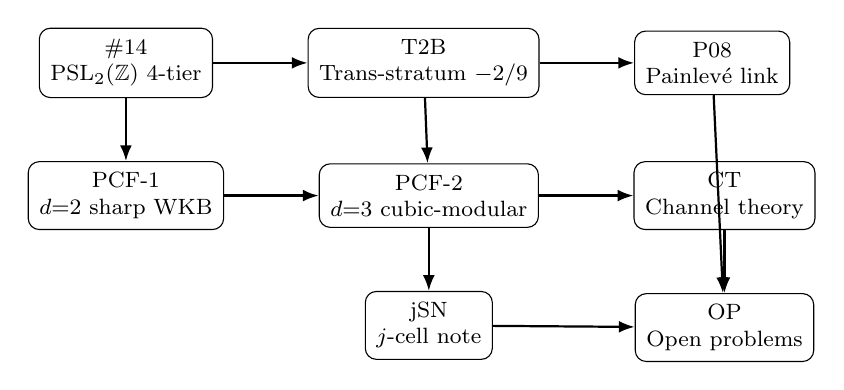
\begin{tikzpicture}[
  node distance=8mm and 12mm,
  every node/.style={draw, rounded corners, align=center,
                     font=\footnotesize, inner sep=4pt},
  arr/.style={-{Latex[length=2mm]}, thick}
]
\node (p14) {\#14\\ $\PSLZ$ 4-tier};
\node (t2b) [right=of p14] {T2B\\ Trans-stratum $-2/9$};
\node (p08) [right=of t2b] {P08\\ Painlev\'e link};
\node (pcf1)[below=of p14] {PCF-1\\ $d{=}2$ sharp WKB};
\node (pcf2)[right=of pcf1] {PCF-2\\ $d{=}3$ cubic-modular};
\node (ct)  [right=of pcf2] {CT\\ Channel theory};
\node (jsn) [below=of pcf2] {jSN\\ $j$-cell note};
\node (op)  [below=of ct]  {OP\\ Open problems};

\draw[arr] (p14) -- (t2b);
\draw[arr] (t2b) -- (p08);
\draw[arr] (pcf1) -- (pcf2);
\draw[arr] (pcf2) -- (ct);
\draw[arr] (p14)  -- (pcf1);
\draw[arr] (t2b)  -- (pcf2);
\draw[arr] (pcf2) -- (jsn);
\draw[arr] (ct)   -- (op);
\draw[arr] (p08)  -- (op);
\draw[arr] (jsn)  -- (op);
\end{tikzpicture}
\caption{Dependency graph of the SIARC companion papers (v2.0).
Arrows denote ``logical prerequisite''; the umbrella paper (this
document, v2.0) sits above all nodes and provides the unified
notation and the cross-degree invariant triple of
\S\ref{sec:triple}.}
\label{fig:depgraph}
\end{figure}

\subsection{Unified notation}

Across the series we adopt the following conventions. Companion papers
that predate this umbrella may use slightly different notation locally;
the table below is the canonical reference and absorbs the v2.0
additions (the invariant triple, the channel and bridge functors, the
cell decomposition, and the residual notation).

\begin{center}
\begin{tabular}{@{}lll@{}}
\toprule
Symbol & Meaning & Convention \\
\midrule
$x$ & PCF variable & integer, $x \geq 1$ \\
$a_n(x), b_n(x)$ & partial num./denom.\ polynomials & $\Z[x]$ \\
$(d_a, d_b)$ & degree pair & $d_a = \deg a_n$, $d_b = \deg b_n$ \\
$d$ & denominator polynomial degree & $d = \deg b$ (cross-degree label) \\
$\Gamma$ & uniformizing Fuchsian group & subgroup of $\PSLZ$ unless stated \\
$K(x)$ & limit of the PCF at $x$ & in $\R \cup \{\infty\}$ \\
$\mu(\alpha)$ & irrationality measure of $\alpha$ & $\mu \geq 2$ for irrationals \\
$c_{\Gamma,(d_a,d_b)}$ & trans-stratum exponent & rational, depends on $\Gamma$ and degrees \\
T0--T3 & arithmetic tiers & as in \S\ref{sec:tiers} \\
$\Delta_d(b)$ & polynomial discriminant axis & $\mathrm{disc}(b)$, $\S$\ref{sec:triple-disc} \\
$\tau_b$ & period of $E_b: y^2 = b(x)$ & in $\HH/\mathrm{SL}_2(\Z)$ \\
$\PetN{\Delta}(\tau_b)$ & Petersson modular-discriminant axis & $|\Delta(\tau_b)|(\mathrm{Im}\,\tau_b)^6$ \\
$\xi_0(b)$ & Borel-radius axis & $d/\beta_d^{1/d}$, $\S$\ref{sec:triple-borel} \\
$E,\ P_k,\ B$ & cell decomposition & $\S$\ref{sec:triple-cells} \\
$\chi$ & channel functor & \cite{CT} \\
$\Phi$ & bridge functor (umbrella v2.0) & \eqref{eq:Phi-functor} \\
$\delta_n$ & PCF residual (PCF-2 notation) & $\delta_n = \log|p_n - K(x) q_n|$ \\
$A_{\mathrm{fit}}, A_{\mathrm{PCF}}$ & fitted and conjectured WKB exponent & $A_{\mathrm{PCF}} = 2d$ (Conj.~B4) \\
\bottomrule
\end{tabular}
\end{center}

\noindent
\textbf{Degree convention.} Throughout the series, ``degree-$(d_a, d_b)$''
refers to the \emph{generic} polynomial degrees of $a_n$ and $b_n$ as
functions of the index $n$ in the underlying recurrence, not as
functions of $x$. A degree-$(2,1)$ family is therefore one in which
the numerator polynomial grows quadratically in $n$ and the denominator
grows linearly in $n$. The cross-degree label $d = \deg b$ of
\S\ref{sec:triple} matches $d_b$ at $\PCF(1,b)$ where $\deg a = 0$.

\paragraph{Coefficient ordering.} PCF family coefficients
$[a_2, a_1, a_0, b_1, b_0]$ and $[\beta_d, \dots, \beta_0]$ are stored
\emph{leading-coefficient-first} throughout the SIARC stack
(\texttt{f1\_base\_computation.py} convention). This matches the v2.0
notation: $\xi_0(b) = d/\beta_d^{1/d}$ uses $\beta_d$ as the leading
coefficient of $b$.

\section{The Trans-Stratum Conjecture}
\label{sec:t2b}

The single most distinctive empirical phenomenon of the program is
the persistent appearance of the rational exponent $-2/9$ in the
trans-stratum of degree-$(2,1)$ families uniformized by $\PSLZ$.

\begin{conjecture}[Trans-stratum two-class conjecture]
\label{conj:t2b}
Let $\{K(x)\}$ be a PCF family of generic degree $(2,1)$
uniformized by $\PSLZ$, satisfying the regularity conditions
of companion paper~T2B.  Then $K(x)$ lies in tier T2 and falls
into exactly one of two classes, distinguished by the
structural ratio $\rho := a_2/b_1^2$:
\begin{itemize}
  \item Class A ($\rho = -2/9$): trans-stratum exponent
        $c_{\PSLZ,(2,1),A} = -2/9$ (T2B Theorem~2,
        conditional on $S_{12}\neq 0$);
  \item Class B ($\rho = +1/4$): limits lie in
        $\mathbb{Q}(\pi)$ (T2B Theorem~3); the Pure-regime
        subclass satisfies the stronger $\mathbb{Q}\cdot\pi^{-1}$
        (T2B Cor.~classB-pi).
\end{itemize}
Equivalently (T2B Completeness Conjecture): the degree-$(2,1)$
Trans-stratum is exactly $\mathcal{T}_A \sqcup \mathcal{T}_B$,
with no third class.
\end{conjecture}

\begin{remark}[Pre-revision form]
\label{rem:t2b-prerev}
The version of this conjecture in UMB v1 (Zenodo
\href{https://doi.org/10.5281/zenodo.19885550}{10.5281/zenodo.19885550})
stated only the Class A clause.  The current form incorporates the
Class B census of companion paper~T2B (16 canonical families,
height $\leq 100$).  No previously asserted Class A claim is revoked;
the change is purely additive.
\end{remark}

\begin{remark}[Empirical basis]
\label{rem:empirical}
A computational census reported in companion paper~T2B
(Zenodo concept DOI \href{https://doi.org/10.5281/zenodo.19783311}{10.5281/zenodo.19783311})
covers approximately $150{,}000$ degree-$(2,1)$ families generated
under the regularity conditions of that paper. Across the entire
census, no counterexample to Conjecture~\ref{conj:t2b} has been
observed; the empirical fit to the predicted $-2/9$ slope is consistent
with the reported numerical precision. We do not reproduce the
empirical methodology, the regularity conditions, or any proof
attempt in this document; all such material lives in T2B.
\end{remark}

\begin{remark}[Why $-2/9$?]
The value $-2/9$ arises in companion paper~T2B via the
indicial exponents $\{1/3, 2/3\}$ of the associated
three-term recurrence at infinity: the ratio $a_2/b_1^2$
is determined by requiring the indicial roots to sum to
$1$ and multiply to $2/9$, giving $1/3 + 2/3 = 1$ and
$(1/3)(2/3) = 2/9$. A congruence-subgroup interpretation
of this denominator is speculative and not established;
a rigorous derivation from the monodromy of the
uniformizing group remains the central open problem.
\end{remark}

\begin{remark}[Projective verification of Conjecture~\ref{conj:t2b}, Class A]
\label{rem:projective-verify}
A targeted projective-coordinate sweep
($H = 8$, $b_1 \in \{3, 6, \ldots, 30\}$ subject to $3 \mid b_1$,
$48{,}552$ primitive 5-tuples
$(a_2, a_1, a_0, b_1, b_0)$ satisfying $9 a_2 + 2 b_1^2 = 0$,
$\gcd = 1$, $b_1 > 0$; $43{,}915$ distinct-$L$ families;
stratified random sample of $400$ groups, $40$ per $b_1$ bucket)
confirms the Class A clause of Conjecture~\ref{conj:t2b}
empirically: $387/400$ sampled families are Trans, with
$0$ Log, $0$ Alg, $13$ rational, and $0$ phantom hits
under PSLQ at \texttt{dps}$=400$, $\mathrm{tol} = 10^{-50}$,
basis $\{1, \pi, \pi^2, \log 2, \zeta(2), \zeta(3),
\sqrt{2}, \sqrt{3}, \sqrt{5}, e, \gamma, \log 3,
\pi \log 2, \pi^2, \pi^3\}$, with mandatory rejection of any
relation whose $L$-coefficient vanishes. The smallest
witness is
$(a_2, a_1, a_0, b_1, b_0) = (-2, 0, 1, 3, -1)$ with
$L \approx 0.26057$. An earlier affine-coordinate
enumeration at fixed height $H = 5$
($b_1 \in \{9, 12, 15, 30\}$) found $0$ Trans families;
the discrepancy is a coordinate artefact resolved by passing
to projective normalization with $\gcd = 1$ and $b_1 > 0$,
which admits primitive small-coefficient witnesses
(in particular $b_1 = 3$ with $|a_1|, |a_0|, |b_0| \leq 1$)
that are absent from any fixed-height affine slice.
Every $3 \mid b_1$ bucket in the sample contains at least
$32$ Trans families. Full numerics, classifier source, and
sample data are recorded in
\texttt{sessions/2026-04-30/UMB-RES-EXTEND-PROJ/} of the
SIARC relay bridge repository.
\end{remark}

\paragraph{Cross-degree extension.}
\label{par:t2b-cross-degree}
The Trans-Stratum two-class conjecture above is the $d=2$
specialisation of the cross-degree framing of \S\ref{sec:triple}.
Class A (rationals, $\rho = -2/9$, Birkhoff--Trjitzinsky resolution)
and Class B (rationals in $\Q(\pi)$, $\rho = +1/4$,
Gauss-continued-fraction / Ramanujan resolution) are recovered as
the two branches of the $\Delta_2$-axis split: $\Delta_2 < 0$ aligns
with Class~A and the BT-resolved tier; $\Delta_2 > 0$ aligns with
Class~B and the GCF/Ramanujan-resolved tier (PCF-1 v1.3
\cite{PCF1}). At $d \geq 3$, the analogous split is the
$\Delta_d$-axis component of the bridge functor $\Phi$ of
\eqref{eq:Phi-functor}; the $\PetN{\Delta}$-axis refinement is
genuinely new at $d=3$ (Conjecture~\ref{conj:b5-b6-d3}). The
v2.0 framing therefore \emph{subsumes} the (2,1)-only Trans-Stratum
Conjecture without retracting any of its content.

\section{Open Problems}
\label{sec:open}

We list the principal open problems of the program in rough order of
expected tractability. Each is stated informally; precise formulations
appear in the indicated companion papers. Problems carried over from
v1 retain their numbering; v2.0 additions follow.

\begin{problem}[Degree-$(3,1)$ classification]
\label{prob:31}
Establish the four-tier classification for $\PSLZ$-uniformized PCF
families of generic degree $(3,1)$. The asymmetry between numerator and
denominator degrees breaks the symmetric treatment of \#14.
\emph{Status (v2.0):} the structural-correlation half of the problem is
substantially answered at $d=3$ by PCF-2 v1.3 \cite{PCF2} and the
cubic-modular framing of \S\ref{sec:triple-moddisc} (R1.1 / T2 verdicts);
the rigorous-classification half remains open. Cross-references:
\textsf{op:b4-degree-d}, \textsf{prob:b4-allD}.
\end{problem}

\begin{problem}[Trans-stratum at $d=2$ for non-$\PSLZ$]
\label{prob:t2-d2-nonpsl}
Determine the trans-stratum exponent $c_{\Gamma,(2,1)}$ for
$\Gamma = \Gamma_0(2)$ and for the Hecke triangle groups $G_q$ with
$q \geq 4$. Is the value $-2/9$ specific to $\PSLZ$, or does it
recur with a $\Gamma$-dependent denominator?
\emph{Status (v2.0):} unchanged; the $\Gamma_0(2)$ sweep
(\texttt{sessions/2026-04-30/UMB-GAMMA0-2-SWEEP/}) supplies a
preliminary census but no exponent identification.
\end{problem}

\begin{problem}[Painlev\'e connection]
\label{prob:painleve}
Make precise the conjectural correspondence between trans-stratum PCF
families and solutions of Painlevé~VI with monodromy in $\Gamma$.
A pointer-level discussion is given in companion paper~P08; a full
correspondence theorem is open.
\end{problem}

\begin{problem}[Effective T0/T1 boundary]
\label{prob:effective}
Provide an algorithm that, given the polynomials $a_n(x), b_n(x)$ in
exact arithmetic, decides in finite time whether the family lies in
T0 or T1. \#14 establishes the boundary as a set; effectivity is open.
\end{problem}

\begin{problem}[T3 nonemptiness]
\label{prob:t3}
Exhibit an explicit PCF family that provably lies in T3 (not merely
fails to lie in T0--T2 by current methods). Equivalently, exhibit a
PCF whose monodromy group has infinite covolume in a controlled way.
\end{problem}

\begin{problem}[Mahler--Nesterenko gap]
\label{prob:mahler}
For T1 families, identify the precise hypothesis that fails when the
Mahler criterion does not apply and the Nesterenko criterion does.
The empirical gap is small; a structural explanation is missing.
\end{problem}

\begin{problem}[Census completeness]
\label{prob:census}
Extend the empirical census underlying Conjecture~\ref{conj:t2b}
beyond degree-$(2,1)$. A negative result --- a single counterexample
in any degree --- would falsify the Trans-Stratum Conjecture as
stated and force a refinement.
\end{problem}

\paragraph{New problems introduced by v2.0.}

\begin{problem}[Conjecture B4 at all $d$ via Birkhoff--Trjitzinsky]
\label{prob:b4-allD}
Establish $A_{\mathrm{PCF}}(b) = 2d$ for all $d$ and all
irreducible non-singular $b \in \Q[x]$ with $\deg b = d$, in the
sharp form of \eqref{eq:b4-conjecture}. PCF-1 v1.3 verifies $d=2$;
PCF-2 v1.3 verifies $d \in \{3, 4\}$ on $110/110$ families. The
strong-form upgrade follows the Birkhoff--Trjitzinsky asymptotic
theory of irregular linear difference equations \cite{Birkhoff1930,
BirkhoffTrjitzinsky1933}; this is the gating move toward the
SIARC Master Conjecture v0.
Tag: \textsf{op:b4-degree-d}.
\end{problem}

\begin{problem}[Modular-discriminant stratification at $d=3$]
\label{prob:modular-discriminant-stratification}
Make precise the conjectural claim that $\PetN{\Delta}(\tau_b)$
stratifies the $d=3$ cubic catalogue beyond the bare $j$-invariant.
Identify the modular-form weight at which the stratification
becomes sharp (in particular: is the weight-$12$ Petersson
discriminant the asymptotic optimum, or does a higher-weight cusp
form refine it further?). Cross-references: \cite{PCF2} Session~T2,
Conjecture~\ref{conj:b5-b6-d3}.
\end{problem}

\begin{problem}[Closed-form $j=0$ amplitude (Chowla--Selberg)]
\label{prob:j-zero-amplitude}
Closed-form expression for the cubic $A=6$ subleading amplitude
at the equianharmonic CM cell ($j=0$, $\tau = \rho =
e^{2\pi i/3}$), conjectured to involve a Chowla--Selberg
$\Gamma(1/3)$ basis element \cite{ChowlaSelberg1967}. Recommended
protocol: redesigned five-parameter WKB ansatz at $\mathrm{dps}
\geq 8000$, $N_{\max} \geq 1200$, with explicit Chowla--Selberg
target basis. Tag: \textsf{op:j-zero-amplitude-h6} (relay
\textsf{T2.5d}).
\end{problem}

\begin{problem}[$j=1728$ wedge]
\label{prob:j-1728-wedge}
Order-$2$ elliptic-point CM-locus probe at $d=3$, $j=1728$:
quantify the residual $\PetN{\Delta}$-axis signal at the
$E_6(\tau_b) = 0$ wedge after the $E_4$-zero ($j=0$) cell is
removed. Tag: \textsf{op:j-1728-wedge} (relay \textsf{T2.5b}).
\end{problem}

\begin{problem}[Shallow-$N$ $j=0$ effect at $d=4$]
\label{prob:shallow-j-effect-d4}
The shallow-$N$ $j=0$ cell shift at $d=4$ is highly significant
($p = 1.1\times 10^{-6}$ stratified) but dissolves at deep $N$.
Identify the sub-leading WKB term ($\beta \log N$ or $\gamma$) that
carries this shallow signal, and decide whether it lifts to a
deep-$N$ rule under any precision/window enlargement. Tag:
\textsf{op:shallow-j-effect-d4}.
\end{problem}

\begin{problem}[Painlev\'e cells $P_k$ as substrata of $\mathcal{M}_{1,1}$]
\label{prob:Pk-cells-structure}
Characterise the Painlev\'e-reduction cells $P_k$ of
\S\ref{sec:triple-cells} as substrata of the moduli space
$\mathcal{M}_{1,1}$ (or its degree-$d$ generalisation). Fleet-A
H3 status: \textsf{D=2\_REDUCTION\_AMBIGUOUS} (the $P_2$ cell at
$d=2$ admits more than one Painlev\'e parametrisation under the
current criteria).
\end{problem}

\begin{problem}[Median-resurgence extension beyond V$_{\mathrm{quad}}$]
\label{prob:median-resurgence-extension}
Extend the median-resurgence framework of Channel Theory v1.2
\cite{CT} from the V$_{\mathrm{quad}}$ stratum to the cubic
CC channels. Fleet-A H4 confirmed $\geq 30$-digit recovery on
V$_{\mathrm{quad}}$; the cubic-CC analogue is open. Tag:
\textsf{op:median-resurgence-extension}.
\end{problem}

\begin{problem}[Compatibility of $\chi$ and $\Phi$]
\label{prob:chi-Phi-compatibility}
Establish that the bridge functor $\Phi$ of \eqref{eq:Phi-functor}
factors through the channel functor $\chi$ of \cite{CT} in a way
compatible with the cell decomposition $E / P_k / B$ of
\S\ref{sec:triple-cells}. Tag: \textsf{op:chi-Phi-compatibility}.
\end{problem}

\paragraph{Problems closed since v1.}
\textsf{op:finer-cubic-split} (resolved by PCF-2 v1.3 cubic-modular
framing; closed in \cite{PCF2}). The resolution is
Conjecture~\ref{conj:b5-b6-d3} above.

\section{Companion Papers and Status}
\label{sec:companions}

The table below records the current state of the SIARC series at the
time of this v2.0 umbrella draft. DOIs marked ``--'' are not yet
issued; ``TBA'' is pending. Statuses are intended to be updated in
revisions of this document.

\begin{center}
\renewcommand{\arraystretch}{1.15}
\begin{longtable}{@{}p{0.10\linewidth} p{0.32\linewidth} p{0.22\linewidth} p{0.28\linewidth}@{}}
\toprule
ID & Title (working) & Venue / status & Zenodo concept / version DOI \\
\midrule
\endfirsthead
\toprule
ID & Title (working) & Venue / status & Zenodo concept / version DOI \\
\midrule
\endhead
\multicolumn{4}{@{}l}{\emph{Published (Zenodo, May 2026)}} \\
\midrule
PCF-1 & Polynomial continued fractions at degree $(d,1)$: sharp WKB exponents and an arithmetic stratification & Zenodo v1.3 (2026-05-01); Compositio CM~10573 in review & \href{https://doi.org/10.5281/zenodo.19937196}{10.5281/zenodo.19937196} (v1.3) / concept \href{https://doi.org/10.5281/zenodo.19931635}{19931635} \\
PCF-2 & Polynomial continued fractions at degree three: a cubic-modular framing & Zenodo v1.3 (2026-05-02); program statement, 22pp & \href{https://doi.org/10.5281/zenodo.19963298}{10.5281/zenodo.19963298} (v1.3) / concept \href{https://doi.org/10.5281/zenodo.19936297}{19936297} \\
CT    & Channel Theory: V$_{\mathrm{quad}}$ resurgence and the CC-pipeline & Zenodo v1.2 (2026-05-01) & \href{https://doi.org/10.5281/zenodo.19951331}{10.5281/zenodo.19951331} (v1.2) / concept \href{https://doi.org/10.5281/zenodo.19941678}{19941678} \\
T2B   & Two arithmetic classes of degree-$(2,1)$ Trans-stratum continued fractions: a Birkhoff--Trjitzinsky / Gauss-continued-fraction dichotomy & Zenodo v3.0 (2026-04-30) & \href{https://doi.org/10.5281/zenodo.19915689}{10.5281/zenodo.19915689} (v3.0) / concept \href{https://doi.org/10.5281/zenodo.19783311}{19783311} \\
UMB   & \emph{This document} (umbrella program statement, v2.0) & Zenodo v2.0 (this version) & concept \href{https://doi.org/10.5281/zenodo.19885550}{10.5281/zenodo.19885550} (v1 superseded) \\
\midrule
\multicolumn{4}{@{}l}{\emph{Drafting / forthcoming}} \\
\midrule
jSN   & The $j$-invariant cell of degree-$3$ PCFs (standalone note, 4pp) & Polished; arXiv submission forthcoming & arXiv: TBA \\
D1    & Cubic--quartic results paper & Drafting (post-PCF-2 v1.3) & -- \\
D2-NOTE & Newton-polygon universality of $\xi_0 = d/\beta_d^{1/d}$ & Drafting & -- \\
D3    & Channel-theory results paper & Planned (post-CT v1.3) & -- \\
D7    & AEAL methodology for verified experimental mathematics at scale & Drafting & -- \\
MASTER-V0 & SIARC Master Conjecture v0 announcement & Planned (post-T1 / Birkhoff--Trjitzinsky) & -- \\
\midrule
\multicolumn{4}{@{}l}{\emph{Carried over from v1 (status updated)}} \\
\midrule
\#14 & Four-tier classification of $\PSLZ$-uniformized PCFs & Submitted; under revision after two desk-rejects on citation hygiene & TBA (post-acceptance) \\
P08  & Painlev\'e~VI and trans-stratum PCFs (pointer paper) & Draft & -- \\
G1   & Extension of the four-tier hierarchy to $\Gamma_0(2)$ & Draft & -- \\
G2   & Trans-stratum exponents for Hecke triangle groups & Outline & -- \\
OP   & Open-problems census for the SIARC program & Outline; superseded by \S\ref{sec:open} of this paper & -- \\
\bottomrule
\end{longtable}
\end{center}

\paragraph{Note on proofs.}
By design, no proof from any of the above papers is reproduced in this
document. Where a claim in this document would require proof, it has
been stated as a conjecture, an open problem, or a remark with a pointer
to the responsible companion paper. Readers seeking proofs should
consult the cited companion paper directly.

\section{AI Disclosure}
\label{sec:ai}

This v2.0 umbrella absorbs the post-March 2026 SIARC stack, which was
produced via a \emph{multi-agent fleet methodology}: parallel sessions
for hypothesis-testing (the Fleet-A unification stack), audit fleets
(Fleet-F), AEAL claim chains (per-session
\texttt{claims.jsonl} files mirrored on the SIARC relay bridge
\href{https://github.com/papanokechi/siarc-relay-bridge}{github.com/papanokechi/siarc-relay-bridge}),
and rubber-duck critique passes on every release. All
\emph{mathematical content} in this document --- definitions,
conjectures, open problems, the structure of the program, the assignment
of claims to companion papers, and the precise form of the cross-degree
invariant triple of \S\ref{sec:triple} --- was determined by the author.
The LLM tooling (GitHub Copilot powered by Anthropic Claude Opus~4.7,
and standalone Anthropic Claude sessions) produced LaTeX scaffolding,
numerical orchestration, build-log parsing, and copy-editing under
direct human supervision; no part of the empirical census underlying
Conjecture~\ref{conj:t2b} or the Petersson-discriminant correlation of
\S\ref{sec:triple-moddisc} was generated by a language model. Those
numbers are the product of the deterministic computational pipelines
described in T2B and PCF-2 v1.3, and are reproducible from the session
deliverables on the SIARC bridge.

The AEAL claim schema --- formalised in PCF-2 v1.3 (\cite{PCF2}, the
``AEAL schema (v1.3 canonical form)'' paragraph; addresses Fleet-F
audit finding F1-01) --- is the canonical schema across the program
from v1.3 forward, and is the schema used in the
\texttt{sessions/2026-05-02/SIARC-UMBRELLA-V2-RELEASE/claims.jsonl}
companion to this release. The author reviewed and takes full
responsibility for every statement in this document.

\section*{Acknowledgments}
The author thanks the maintainers of the Zenodo platform for providing
a stable DOI infrastructure that makes a program-paper of this kind
possible. v2.0 absorbs SIARC sessions PCF1-* (P12 / Compositio prep,
January--April 2026), PCF2-* (R1.1, R1.2, R1.3, T2, V12-RELEASE,
V13-RELEASE, May 2026), and the triple-fleet audit
(Fleet-A, Fleet-F, standalone-note polish, May 2026). The author
thanks the GitHub Copilot CLI multi-agent fleet for the synthesis,
audit, and assembly support during the v1$\to$v2.0 refactor.

\begin{thebibliography}{99}

\bibitem{PCF1}
papanokechi,
\emph{Polynomial continued fractions at degree $(d,1)$: sharp WKB exponents and an arithmetic stratification}
(SIARC companion paper PCF-1),
Zenodo preprint, v1.3, 2026-05-01.
Version DOI: \href{https://doi.org/10.5281/zenodo.19937196}{10.5281/zenodo.19937196};
concept DOI: \href{https://doi.org/10.5281/zenodo.19931635}{10.5281/zenodo.19931635}.
Compositio Mathematica CM~10573 (in review).

\bibitem{PCF2}
papanokechi,
\emph{PCF-2: Polynomial Continued Fractions at Degree Three --- v1.3 (Cubic-Modular Framing)}
(SIARC companion paper PCF-2),
Zenodo preprint, v1.3, 2026-05-02.
Version DOI: \href{https://doi.org/10.5281/zenodo.19963298}{10.5281/zenodo.19963298};
concept DOI: \href{https://doi.org/10.5281/zenodo.19936297}{10.5281/zenodo.19936297}.

\bibitem{CT}
papanokechi,
\emph{Channel Theory: V$_{\mathrm{quad}}$ resurgence and the CC-pipeline}
(SIARC companion paper CT),
Zenodo preprint, v1.2, 2026-05-01.
Version DOI: \href{https://doi.org/10.5281/zenodo.19951331}{10.5281/zenodo.19951331};
concept DOI: \href{https://doi.org/10.5281/zenodo.19941678}{10.5281/zenodo.19941678}.

\bibitem{T2B}
papanokechi,
\emph{Two arithmetic classes of degree-$(2,1)$ Trans-stratum continued fractions: a Birkhoff--Trjitzinsky / Gauss-continued-fraction dichotomy}
(SIARC companion paper T2B),
Zenodo preprint, v3.0, 2026-04-30.
Version DOI: \href{https://doi.org/10.5281/zenodo.19915689}{10.5281/zenodo.19915689};
concept DOI: \href{https://doi.org/10.5281/zenodo.19783311}{10.5281/zenodo.19783311}.

\bibitem{jSN}
papanokechi,
\emph{The $j$-invariant cell of degree-$3$ polynomial continued fractions} (SIARC standalone note, 4pp),
arXiv preprint, math.NT, forthcoming.

\bibitem{Paper14}
papanokechi,
\emph{Four-tier classification of $\PSLZ$-uniformized polynomial continued fractions}
(SIARC companion paper \#14),
submitted; DOI to be assigned upon acceptance.

\bibitem{P08}
papanokechi,
\emph{Painlev\'e~VI and trans-stratum polynomial continued fractions}
(SIARC companion paper P08),
draft; DOI to be assigned.

\bibitem{Birkhoff1930}
G.~D. Birkhoff,
\emph{Formal theory of irregular linear difference equations},
Acta Mathematica \textbf{54} (1930), 205--246.

\bibitem{BirkhoffTrjitzinsky1933}
G.~D. Birkhoff and W.~J. Trjitzinsky,
\emph{Analytic theory of singular difference equations},
Acta Mathematica \textbf{60} (1933), 1--89.

\bibitem{ChowlaSelberg1967}
S.~Chowla and A.~Selberg,
\emph{On Epstein's zeta-function},
Journal f\"ur die reine und angewandte Mathematik \textbf{227} (1967), 86--110.

\end{thebibliography}

\end{document}
